\chapter{Methodology}
We measure one fixed prompt set on every configuration, then evaluate every router by looking up its choices on that measured grid. Because decoding is greedy, each configuration's answer to a prompt does not depend on the routing policy, which makes a policy's energy and correctness exact functions of the measured data.

\section{System architecture}
The system has four layers: a shared workload, two inference stacks, one measurement layer and an offline analysis layer. Stack A quantizes with bitsandbytes~\cite{b20,b21}. Stack B uses vLLM~\cite{b27}, with FP8 support and Marlin kernels for AWQ~\cite{b44,b45}. Holding the workload and meter fixed makes the inference stack the variable under test. Figure 3.1 shows how the layers connect.

\begin{figure}[htbp]
\centering
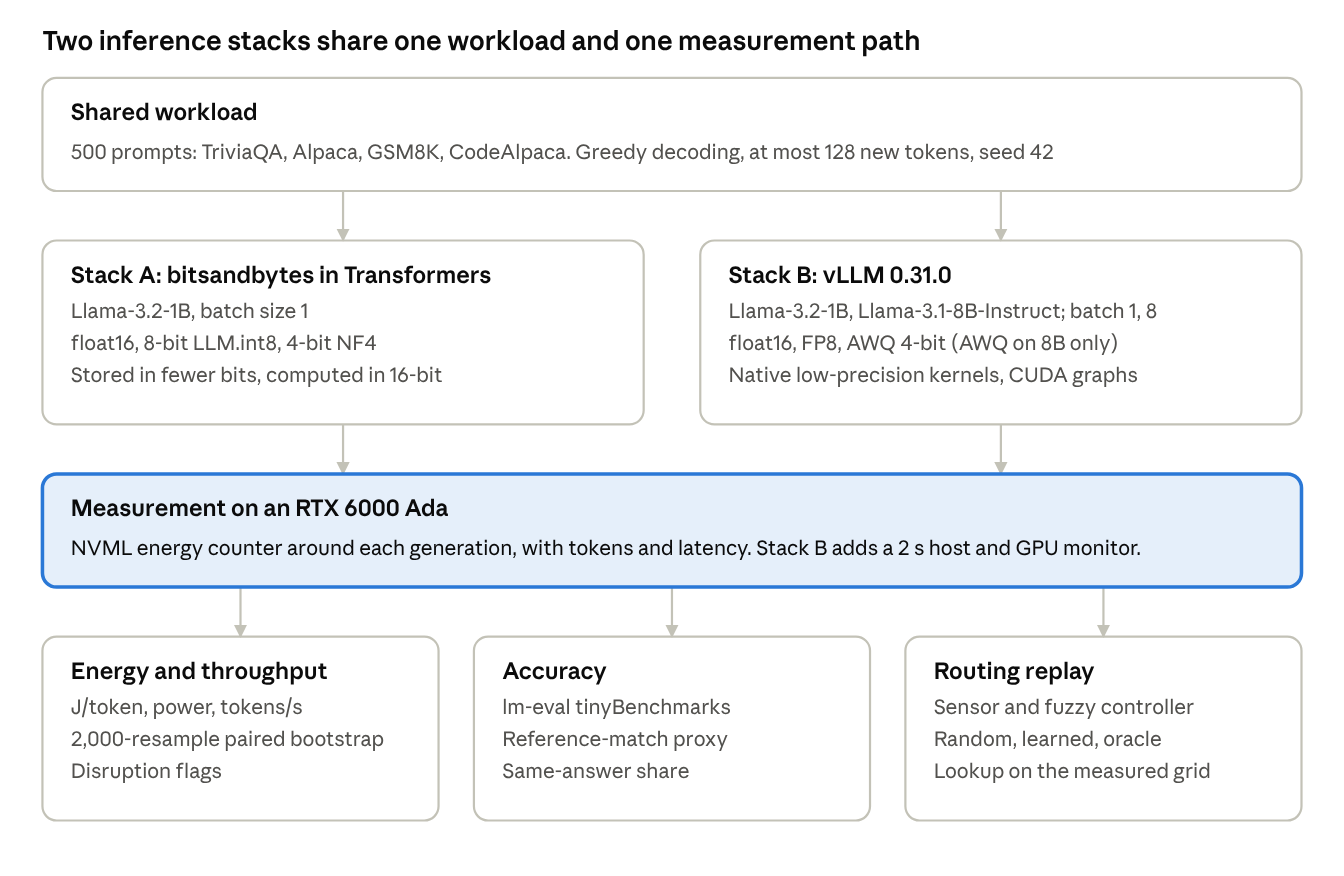
\includegraphics[width=\linewidth]{figs/fig_architecture.png}
\caption[System architecture]{System architecture}
\end{figure}

\section{Experimental workflow}
Every configuration goes through the same steps: warm-up, measurement, logging, then checks. A run enters the analysis only if it passes the disruption check, which we added after finding the pitfall described in section 5.5.

\begin{figure}[htbp]
\centering
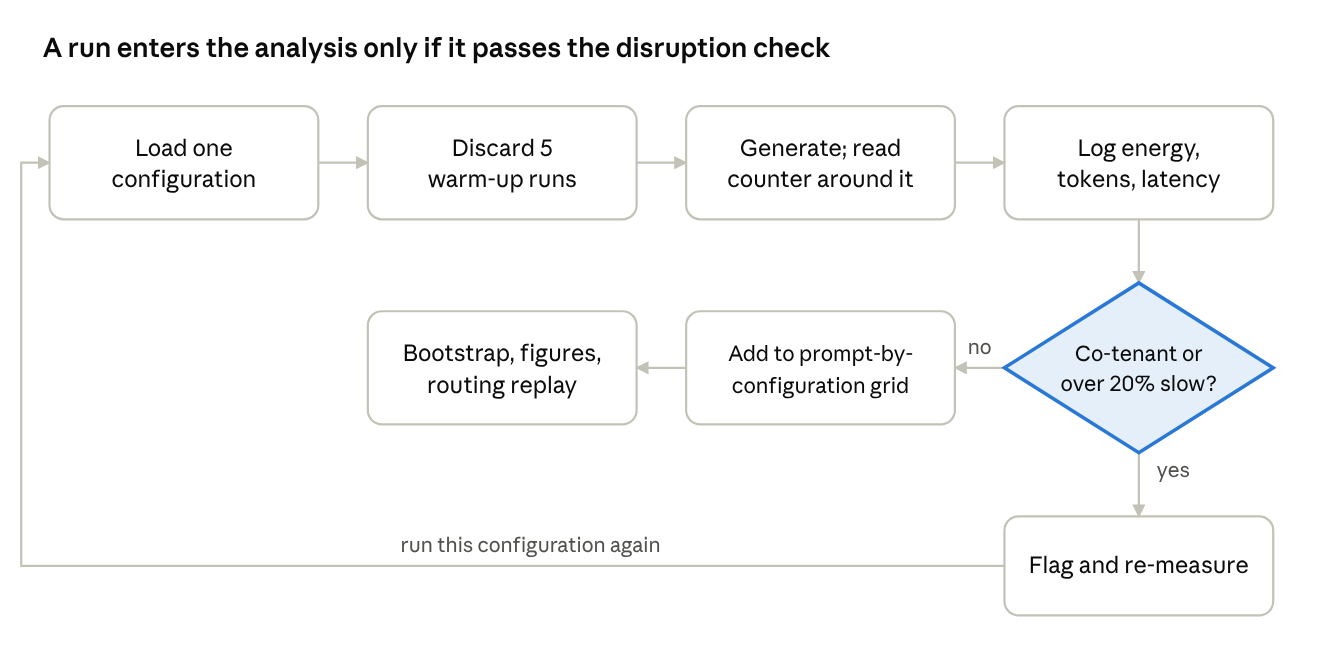
\includegraphics[width=\linewidth]{figs/fig_workflow.png}
\caption[Measurement workflow]{Measurement workflow}
\end{figure}
Stack B applies this check through its monitor and analysis script. Stack A's clean runs had to be identified after the fact from throughput and power, because the check did not yet exist when they were planned.

\section{Modules}

\begingroup\footnotesize\setlength{\tabcolsep}{4pt}
\begin{longtable}{>{\raggedright\arraybackslash}p{32.6mm}>{\raggedright\arraybackslash}p{53.7mm}>{\raggedright\arraybackslash}p{55.3mm}}
\toprule
\textbf{Module} & \textbf{Purpose} & \textbf{Implementation} \\
\midrule
\endhead
Evaluation set builder & Builds 500 unique, stratified prompts; fails rather than pads with duplicates & prepare\_\allowbreak{}eval\_\allowbreak{}dataset.py \\*
Stack A runner & Measures bitsandbytes tiers at batch 1 and computes routing conditions & kaggle\_\allowbreak{}routing\_\allowbreak{}experiment.py \\
Stack B runner & Measures vLLM configurations at batch 1 and 8, with a stall watchdog & vllm\_\allowbreak{}energy\_\allowbreak{}benchmark.py, session5\_\allowbreak{}vllm.sh \\
Energy meter & Reads the GPU's cumulative counter around each generation call & GpuEnergyMeter class (Stack A); Meter class (Stack B) \\
Host monitor & Samples GPU, co-tenant, load and CPU clock data every 2 s (Stack B) & Monitor thread in vllm\_\allowbreak{}energy\_\allowbreak{}benchmark.py \\
Complexity sensor & Computes five normalized prompt features & router/complexity\_\allowbreak{}scorer.py \\
Fuzzy controller & Maps features to a complexity score and a tier & router/fuzzy\_\allowbreak{}controller.py, routellm\_\allowbreak{}bridge.py \\
LoRA adapters & Tier adapters tested for accuracy recovery on Stack A & adapters/, adapter-training.ipynb \\*
Accuracy evaluation & Runs standard benchmarks per configuration & kaggle\_\allowbreak{}accuracy\_\allowbreak{}eval.py, session5\_\allowbreak{}accuracy.sh \\*
Analysis & Bootstrap intervals, routing replay, figures & paper\_\allowbreak{}a\_\allowbreak{}analysis.py, session5\_\allowbreak{}analysis.py, session5\_\allowbreak{}router\_\allowbreak{}replay.py \\*
\bottomrule\noalign{\nobreak}
\end{longtable}
\addtocounter{table}{-1}
\endgroup

Despite its name, routellm\_\allowbreak{}bridge.py is a documented threshold pass-through. It does not load or call a RouteLLM model, because RouteLLM's checkpoints are trained on battles between named models and carry no signal for precision tiers.

\section{Energy measurement}
Energy for a generation call is the change in the GPU's cumulative hardware counter across that call, where $C$ is the NVML reading~\cite{b43} in joules.

\begin{equation}
E_i = C(t_{\mathrm{end}}) - C(t_{\mathrm{start}})
\end{equation}
Throughput and mean power, derived from the same logs, form the basis of the disruption check.

\begin{equation}
T_i = \frac{n_i}{t_i} \qquad\qquad P_i = \frac{E_i}{t_i}
\end{equation}
The two stacks report energy per token differently. Stack A logs each prompt separately, so we take a median over prompts with at least 16 generated tokens. All zero readings came from generations of at most 2 tokens and under 80 ms. The 16-token minimum is a conservative margin: when we varied it from 1 to 64, using non-zero readings, the 4-bit/float16 ratio moved by at most 0.016 within a run and the 8-bit ratio by at most 0.029. Stack B divides total energy by total output tokens, which short generations cannot distort.

\begin{equation}
\text{Stack A: } e = \operatorname{median}_{i:\, n_i \geq 16} \frac{E_i}{n_i}\qquad\qquad \text{Stack B: } e = \frac{\sum_i E_i}{\sum_i n_i}
\end{equation}
In a batched call we attribute energy to prompts in proportion to their output tokens. This is an approximation, since prompts in a batch share one reading, but it does not affect the reported J/token, which uses batch totals, and routing replay uses batch 1.

\begin{equation}
E_i = E_b \cdot \frac{n_i}{\sum_{j \in b} n_j}
\end{equation}
We report each saving against the same model's float16 at the same batch size. Its interval comes from a paired bootstrap over prompts with 2,000 resamples, recomputing the ratio on each resample.

\begin{equation}
\text{saving} = 1 - \frac{e_{\mathrm{config}}}{e_{\mathrm{float16}}}
\end{equation}
\textbf{Algorithm 1: measure one configuration}

\begin{enumerate}
\item Load the configuration, so that it is the only one resident in GPU memory, and record the GPU UUID and driver.
\item Run 5 warm-up generations and discard them.
\item For each prompt or batch, read the counter, generate with greedy decoding up to 128 new tokens, wait for the GPU to finish, and read the counter again. Stack A synchronizes explicitly with torch.cuda.synchronize().
\item Log energy, output tokens, latency, response and correctness for each prompt.
\item On Stack B, sample GPU utilization, power, clocks, co-tenant processes, host load and CPU clock every 2 s throughout, and stop a configuration after 900 s with no progress.
\item Compute energy per token, throughput and mean power, and apply the checks in section 3.2.
\end{enumerate}
\section{Complexity sensor}
The sensor converts a prompt into five features in the range 0 to 1. Continuous features are normalized against fixed ranges calibrated on the 500-prompt set.

\begin{equation}
\hat{x} = \min\!\left(1,\ \max\!\left(0,\ \frac{x - x_{\min}}{x_{\max} - x_{\min}}\right)\right)
\end{equation}

\begingroup\footnotesize\setlength{\tabcolsep}{4pt}
\begin{longtable}{>{\raggedright\arraybackslash}p{36.7mm}>{\raggedright\arraybackslash}p{49.4mm}>{\raggedright\arraybackslash}p{18.3mm}>{\raggedright\arraybackslash}p{34.4mm}}
\toprule
\textbf{Feature} & \textbf{Definition} & \textbf{Range} & \textbf{LOW/MEDIUM and MEDIUM/HIGH edges} \\
\midrule
\endhead
Flesch-Kincaid grade & Readability grade from textstat & 0 to 18 & 5.0, 7.7 \\*
Token length & Characters divided by 4, an approximation & 0 to 154 & 0.086, 0.125 (normalized) \\*
Entropy & Character-level Shannon entropy, in bits & 3.3 to 5.0 & 3.98, 4.16 \\*
Syntax depth & Maximum spaCy dependency-tree depth & 2 to 14 & 4, 5 \\*
Code or maths & 1 for code, LaTeX or maths symbols; code-request words; or two or more numbers with a quantity cue & 0 or 1 & Binary \\*
\bottomrule\noalign{\nobreak}
\end{longtable}
\addtocounter{table}{-1}
\endgroup

The grade and entropy are computed as follows, where $w$, $s$ and $y$ count words, sentences and syllables, and $p_c$ is the share of character $c$.

\begin{equation}
\mathrm{FK} = 0.39\,\frac{w}{s} + 11.8\,\frac{y}{w} - 15.59\qquad\qquad H = -\sum_c p_c \log_2 p_c
\end{equation}
The edges are empirical terciles of each feature on the evaluation set, computed by calibrate\_\allowbreak{}breakpoints.py from the feature values alone, although we did use the difficulty labels when choosing the rule features (section 3.6). We tuned the ranges and edges on the same prompts used for evaluation, a limitation we return to in section 5.8.

\section{Fuzzy controller}
The controller is a Mamdani system built with scikit-fuzzy. MEDIUM is a triangle peaking at the midpoint of the two edges, and LOW and HIGH are saturating trapezoidal shoulders, so a term reaches full membership before the end of the range.

The rule base has 15 rules. Nine cover every combination of terms for the two features that separated the difficulty labels best on this set:


\begingroup\footnotesize\setlength{\tabcolsep}{4pt}
\begin{longtable}{>{\raggedright\arraybackslash}p{52.7mm}>{\raggedright\arraybackslash}p{28.5mm}>{\raggedright\arraybackslash}p{29.0mm}>{\raggedright\arraybackslash}p{28.5mm}}
\toprule
\textbf{Flesch-Kincaid \textbackslash{} Syntax depth} & \textbf{Low} & \textbf{Medium} & \textbf{High} \\
\midrule
\endhead
Low & LOW & LOW & MEDIUM \\*
Medium & MEDIUM & MEDIUM & HIGH \\*
High & MEDIUM & HIGH & HIGH \\*
\bottomrule\noalign{\nobreak}
\end{longtable}
\addtocounter{table}{-1}
\endgroup

Six modifier rules add the other features:

\begin{itemize}
\item Code or maths present gives HIGH.
\item Long length with high readability grade gives HIGH.
\item Long length with medium or low grade gives MEDIUM (two rules).
\item High entropy with high grade gives HIGH.
\item Low grade, short length, low depth and no code gives LOW.
\end{itemize}
Rule strengths use minimum for AND and maximum for aggregation. The output $y$ runs from 0 to 100 with three triangular terms, and centroid defuzzification gives the score $y^{*}$ that selects the tier.

\begin{equation}
y^{*} = \frac{\int y\,\mu(y)\,dy}{\int \mu(y)\,dy}
\end{equation}
\begin{equation}
\text{tier} = \text{low if } y^{*} < 33;\quad \text{middle if } 33 \leq y^{*} \leq 66;\quad \text{high if } y^{*} > 66
\end{equation}
\begin{figure}[htbp]
\centering
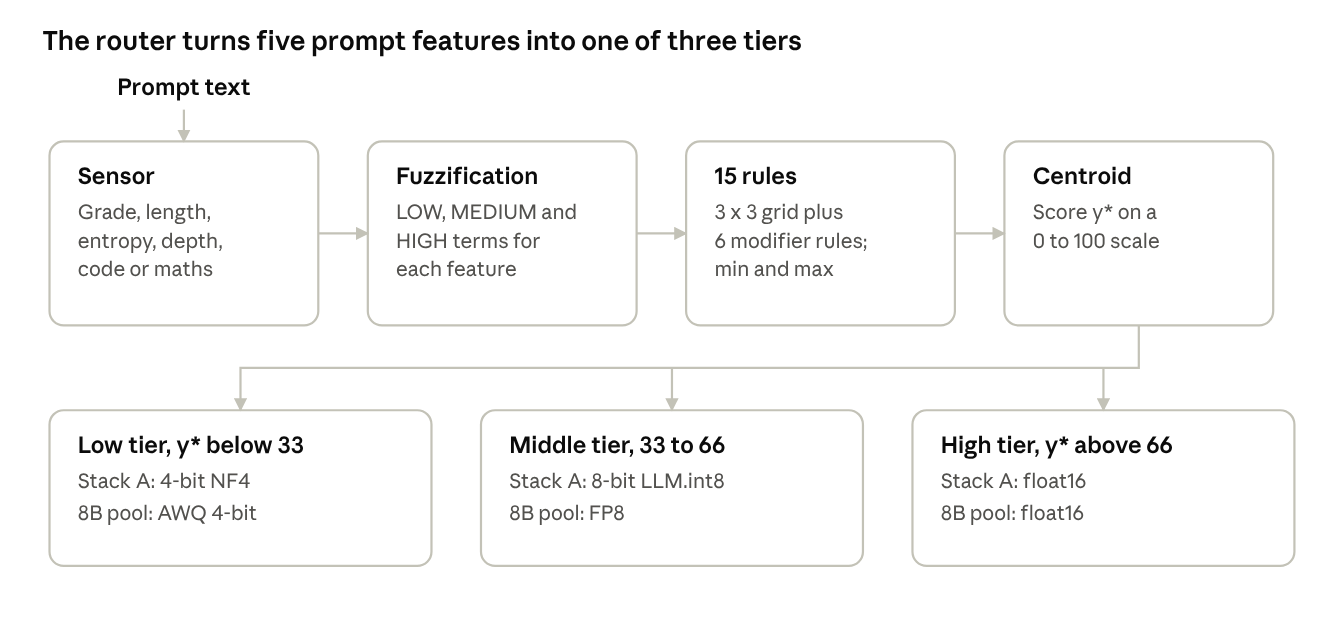
\includegraphics[width=\linewidth]{figs/fig_router.png}
\caption[Router pipeline]{Router pipeline}
\end{figure}
In the two-option 1B/8B pool, the middle and high tiers both map to the larger option.

\textbf{Algorithm 2: route one prompt}

\begin{enumerate}
\item Compute the five raw features of the prompt.
\item Normalize each continuous feature against its fixed range.
\item Fuzzify the features and evaluate all 15 rules.
\item Aggregate the fired output terms and take the centroid $y^{*}$. If no rule fires, set $y^{*} = 50$.
\item Set $w = y^{*}/100$, and return the low tier if $w < 0.33$, the high tier if $w > 0.66$, and the middle tier otherwise.
\end{enumerate}
We reached this design after two rounds of diagnosis. An earlier bridge escalated every score of exactly 50 to 16-bit, and 47\% of prompts scored exactly 50 because no rule discriminated. Fixing both still left 32\% of prompts (161) on the neutral score: 110 from a MEDIUM centroid, and 51 (10.2\%) on which no rule fired and the controller defaulted to 50. Runs 5-7 and all of Session 5 use the corrected router.

\section{LoRA adapters}
We tested three LoRA adapters~\cite{b26} on Stack A to see whether they recover accuracy lost to quantization. They target q\_\allowbreak{}proj and v\_\allowbreak{}proj, with ranks 16, 8 and 4 for the 4-bit, 8-bit and 16-bit tiers, which gives lower precision more capacity. All three were trained on the 4-bit NF4 model, split by a prompt complexity label, so they do not constitute tier-specific quantization-aware training.

\textbf{The adapters are also part of the measured Stack A configurations.} The routing experiment attaches an unmerged adapter to every tier, including float16, in all of runs 1-7; only Session 1 ran without adapters. Stack A energy results therefore describe bitsandbytes with an attached adapter and do not isolate the quantization kernel, a point section 5.1 takes up.

\section{Accuracy and routing evaluation}
We keep two accuracy measures separate. Benchmark accuracy comes from lm-eval-harness on tinyMMLU, tinyHellaswag and tinyGSM8k, with 100 items per task. Routing correctness uses a reference-match proxy on the 500 prompts: numeric match for short numeric answers, normalized substring match for references of up to six words, and stem-level token F1 of at least 0.5 otherwise. Since the proxy is coarse, we interpret only paired differences between policies. tinyGSM8k is reported under flexible-extract scoring, as in the project's logs; strict-match scores are also given in section 5.4, because the choice affects the conclusion.


\begingroup\footnotesize\setlength{\tabcolsep}{4pt}
\begin{longtable}{>{\raggedright\arraybackslash}p{38.3mm}>{\raggedright\arraybackslash}p{59.3mm}>{\raggedright\arraybackslash}p{44.0mm}}
\toprule
\textbf{Policy} & \textbf{Rule} & \textbf{Purpose} \\
\midrule
\endhead
Static & Always one configuration & The baseline a router must outperform \\*
Fuzzy & Algorithm 2 & The system under test \\*
Random-matched & Stack A: exact shuffle of the fuzzy router's tier list, mean of 20 draws. Stack B: random choice with the same mix in expectation, mean of 1,000 draws & Separates routing intelligence from the effect of tier mix \\*
Threshold (Stack A) & The same cuts applied to the plain mean of the five features & Tests what the fuzzy inference adds \\*
Learned (Stack B, 1B/8B pool) & Logistic regression on the same features, predicting whether the cheaper option is correct; 5-fold cross-fitted, thresholds 0.5, 0.7 and 0.9 & Tests one simple learned alternative \\*
Oracle & Stack A: lowest measured energy among correct tiers for that prompt, or lowest overall if none is correct. Stack B: first correct option when ordered by mean energy, or the cheapest on average if none is correct & Indicates the headroom available to routing \\*
\bottomrule\noalign{\nobreak}
\end{longtable}
\addtocounter{table}{-1}
\endgroup

Because the experiment script's own oracle assumed that fewer bits are cheaper, which is false on Stack A, we report the energy-based oracle from the analysis scripts. Only the Stack A form is a per-prompt energy lower bound, which is why the Stack B oracle can cost more than a static tier.

\textbf{Algorithm 3: replay a routing policy}

\begin{enumerate}
\item Build a grid of measured energy and correctness for every prompt and configuration.
\item Score each prompt with the sensor and controller, and map the tiers onto the configurations in the pool.
\item For each policy, select one configuration per prompt and look up its energy and correctness.
\item Report mean energy per request and proxy accuracy, with paired bootstrap intervals against a reference policy.
\end{enumerate}
\section{Statistical analysis}
For energy savings we use a paired bootstrap over prompts, with 2,000 resamples and 95\% percentile intervals, because per-prompt energy need not be normally distributed. Policy comparisons use the same procedure on per-prompt differences. These intervals cover prompt sampling only, not differences in GPU unit, driver or time of day. At batch 8, resampling batches instead of prompts widens them slightly (for example 1B FP8 in run 2, from 36.3--38.6\% to 34.3--40.4\%) without changing the conclusion.

We also computed three further analyses offline from the existing logs, using training/scripts/thesis\_\allowbreak{}extra\_\allowbreak{}analysis.py. They use the same data and involve no new GPU measurement.

\begin{enumerate}
\item \textbf{Accuracy by source dataset.} Paired differences against float16 on each source dataset of the 500 prompts, to check benchmark findings on separate items.
\item \textbf{Threshold sensitivity.} Replay of the fuzzy score at cuts of 25/75, 30/70, 33/66, 40/60 and 45/55, compared with 1,000 random permutations of each resulting tier assignment.
\item \textbf{Feature signal.} Spearman correlation of each feature with correctness and with sensitivity to quantization, where a prompt is sensitive if float16 is correct and the low-precision tier is not. A logistic regression on all five features gives a 5-fold cross-validated AUC.
\end{enumerate}

\section{Reasons for the chosen methodology}

\begingroup\footnotesize\setlength{\tabcolsep}{4pt}
\begin{longtable}{>{\raggedright\arraybackslash}p{38.8mm}>{\raggedright\arraybackslash}p{51.5mm}>{\raggedright\arraybackslash}p{51.3mm}}
\toprule
\textbf{Decision} & \textbf{Reason} & \textbf{Alternative considered} \\
\midrule
\endhead
Hardware energy counter & Measures the GPU directly, without a sampling assumption in the project's own code & Software estimators with coarse sampling, which suit long jobs better than single prompts \\*
One configuration resident at a time & Avoids memory and cache effects from other tiers & Interleaved tiers, tested in run 2, which distribute drift across tiers but were measured under load \\*
Two stacks on one model & Tests whether the outcome depends on implementation & Varying bit-width alone, which hides the implementation effect \\*
vLLM added after Stack A & The research plan named low-bit kernels as the response if bitsandbytes showed no saving & Reframing as a latency study only \\*
Fuzzy controller & Rules are readable and editable; routing added about 10 ms per prompt on the CPU & A learned router alone, retained instead as a baseline \\*
\bottomrule\noalign{\nobreak}
\end{longtable}
\addtocounter{table}{-1}
\endgroup

